
\begin{frame}[ctb!]
  \frametitle{Cyder Paradigm : Modularity }
  A modular repository framework facilitates 
  \begin{itemize}
    \item  interchangable subcomponents (e.g. buffer material) so that 
      the impact on the disposal system performance may be observed
    \item and simulations with varying levels of detail.
  \end{itemize}
 \pause
  Integration with a fuel cycle simulator facilitates
  \begin{itemize}
    \item analysis of feedback effects upon the fuel cycle
    \item and investigation of fuel cycle choices on disposal system 
      performance.
  \end{itemize}
\end{frame}


\begin{frame}[ctb!]
  \frametitle{Cyder Paradigm : Waste Stream Acceptance}
  \footnotesize{
  
To participate in fuel cycle simulation, the repository model must accept arbitrary 
spent fuel and high level waste streams. 
  \begin{figure}[htbp!]
    \begin{center}
      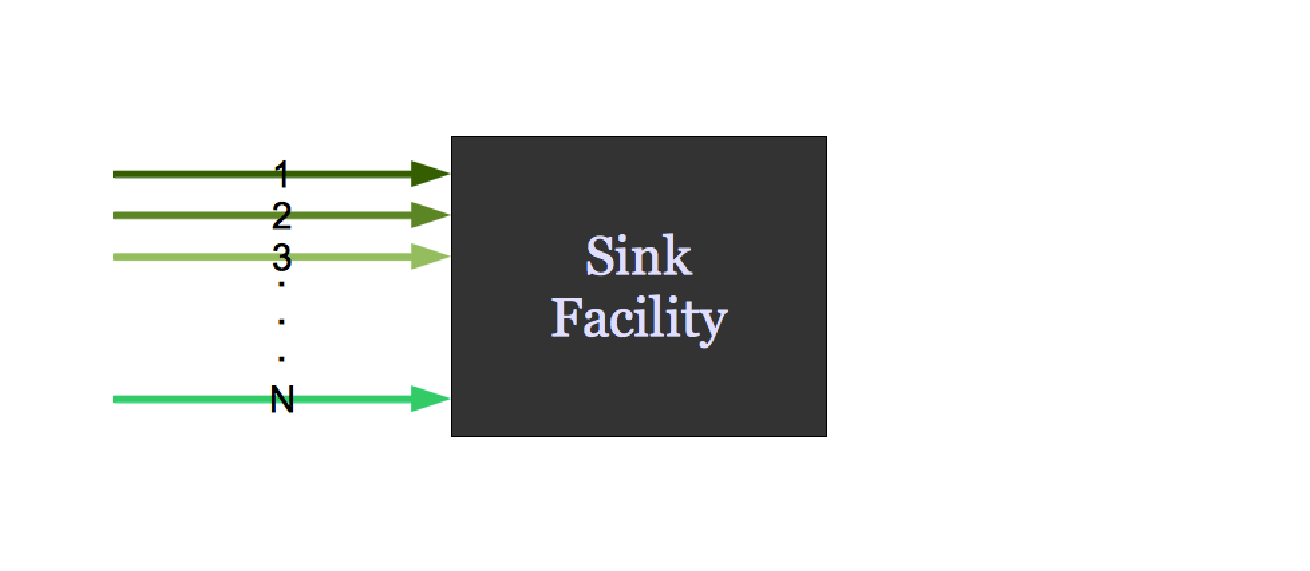
\includegraphics[height=5cm]{./images/sinkfacility.eps}
    \end{center}
    \caption{ The Cyder Facility dynamically accepts material from the coupled 
    fuel cycle simulation.  A waste stream is a material data object resulting 
    from the Cyclus simulated fuel cycle.  } 
    \label{fig:sinkfacility}
  \end{figure}
% Sink Facility ?
}
\end{frame}
